% No modificar estas líneas de código, por favor dirigirse a MARCO INSTITUCIONAL

\newpage

%------------------------
%
%       MARCO INSTITUCIONAL
%
%------------------------

\section{MARCO INSTITUCIONAL}
En el presente capítulo se presenta una visión detallada de la empresa \acrlong{itm}, con énfasis en su historia, misión, visión, valores, así como los productos y servicios que ofrece. Estos elementos proporcionan el contexto institucional necesario para comprender la relevancia de \acrshort{itm} en el desarrollo del proyecto.

\subsection{Historia y origen de la empresa}

\acrshort{itm} es una empresa boliviana fundada en Cochabamba en 2015, con el objetivo de desarrollar soluciones tecnológicas adaptadas al sector de la salud en Bolivia. Desde sus inicios, \acrshort{itm} ha sido pionera en la fabricación y desarrollo de equipos médicos con mano de obra 100\% boliviana, posicionándose como un referente en la gestión de equipamiento médico y tecnología aplicada a hospitales y centros de salud. Durante la pandemia, la empresa jugó un papel crucial al desarrollar prototipos de equipos de esterilización y colaborar en la creación de respiradores funcionales.

\acrshort{itm} ha implementado un Sistema de Gestión de la Calidad certificado bajo la norma ISO 9001:2015, lo que refleja su compromiso con la excelencia y mejora continua. En cuanto a su visión de futuro, \acrshort{itm} busca consolidarse como una empresa internacional de desarrollo tecnológico, con el objetivo de certificar la ISO 13485 para la fabricación de equipos médicos y expandir sus soluciones a nivel internacional.

La empresa está comprometida no solo con la vocación tecnológica, sino también con la generación de empleo local, creando más de 100 empleos directos e indirectos, y con la mejora de los sistemas de salud en Bolivia, enfocándose en resolver problemas locales mediante tecnología propia.
La ubicación de la empresa se encuentra en: Av. Blanco Galindo km 4 1/2 \#3793, como se presenta la fachada en la Figura \ref{fig:emp}.
\begin{figure}[!htb]
    \centering
    \caption{Empresa \acrshort{itm}} % Título de figura
    {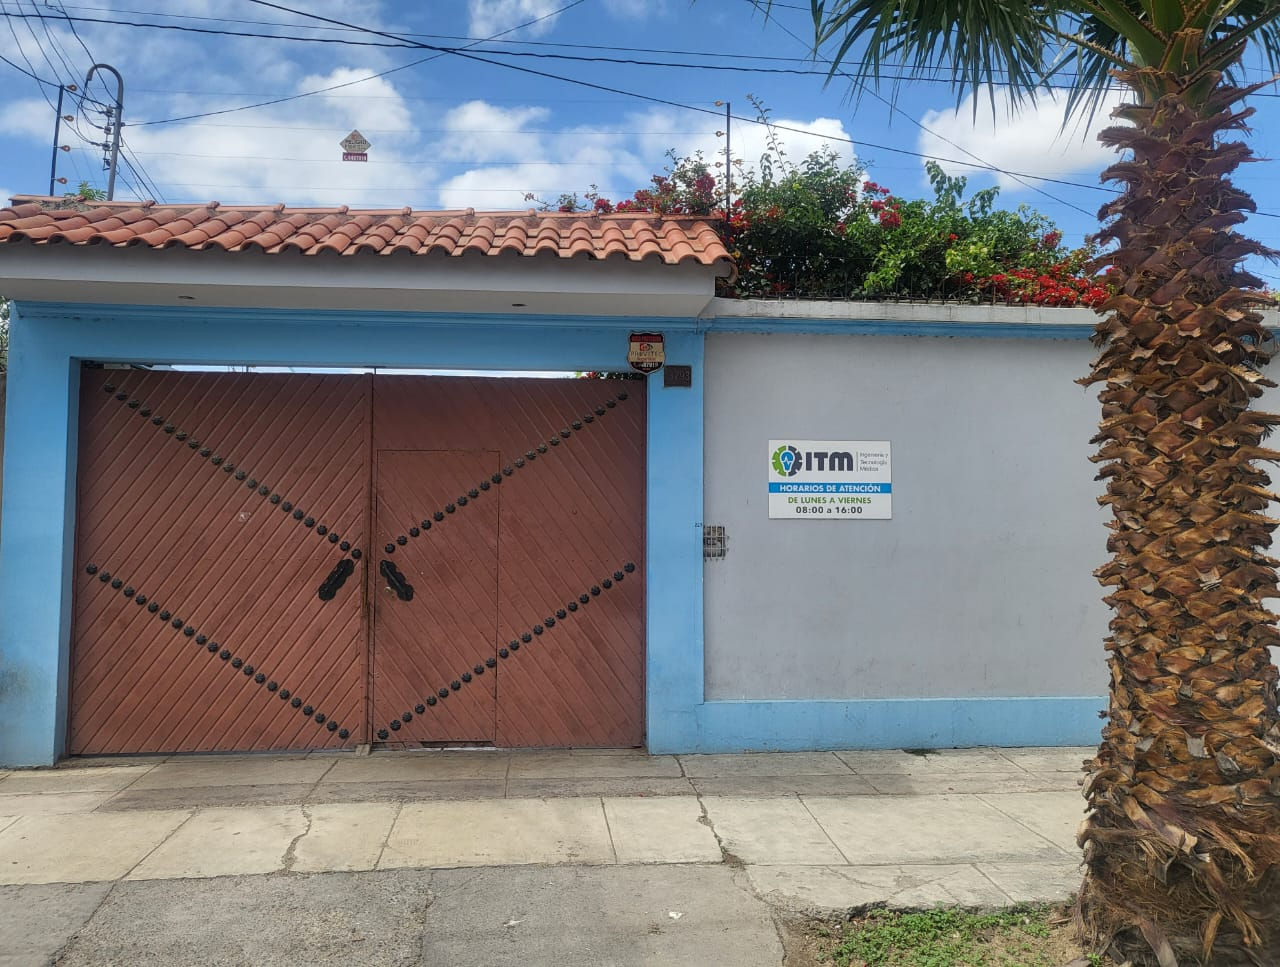
\includegraphics[width=0.6\columnwidth]{Figuras/itm.jpg}}\\
     \centering{\textbf{Fuente:} Elaboración propia (2024)} % Fuente
    \label{fig:emp}
\end{figure}


\subsection{Misión}
Acercar las nuevas tecnologías a la medicina en Bolivia, desarrollando herramientas y servicios con utilidad clínica para mejorar la atención en salud con calidad y calidez, siempre pensando en el beneficio de los pacientes cumpliendo normas nacionales e internacionales.

\subsection{Visión}
Ser la empresa líder a nivel nacional y un referente a nivel internacional en la prestación de servicios y el desarrollo e implementación de tecnologías aplicadas a la ingeniería biomédica para mejorar la atención en salud según normas nacionales e internacionales.

\subsection{Valores}

\begin{itemize}
    \item Responsabilidad - Comprometida con la salud, innovadora, competitiva y orientada a la satisfacción de nuestros clientes.
    \item Pasión - Disfrutamos nuestro trabajo con el entusiasmo y pasión que nos caracteriza como emprendedores.
    \item Compromiso - Buscamos un nuevo nivel de integración multidisciplinario integrando expertos de diferentes áreas profesionales.
    \item Calidad - Mejora continua al ser transparentes con nuestro entorno, buscar la excelencia y el incremento en la satisfacción de nuestros clientes.
\end{itemize}

\subsection{Servicios y productos ofrecidos}
\acrshort{itm} se especializa en el mantenimiento preventivo y correctivo de equipos médicos, asegurando el cumplimiento de requisitos legales y reglamentarios. Su enfoque se centra en el mantenimiento de equipos en hospitales y centros de salud de Cochabamba, destacando su capacidad para ofrecer soluciones tecnológicas adaptadas a las necesidades del sector.

Ofrece una gama de productos diseñados para mejorar la eficiencia en el sector salud, entre los que destacan las autoclaves. Dentro del catálogo, \acrshort{itm} proporciona autoclaves de gran capacidad y de sobremesa como se muestra en la Figura \ref{fig:autoclaves}, ideales para espacios más reducidos, como consultorios médicos, donde se necesita una solución compacta pero igualmente efectiva para la esterilización rápida y segura. Estos productos reflejan el compromiso de la empresa con la innovación y la calidad en el área de la tecnología médica.

\begin{figure}[hpt]
    \centering
    % Título de figura
    \caption{Autoclaves de \acrshort{itm}}
        % imagen 1
        \subfloat[Autoclave ITM]{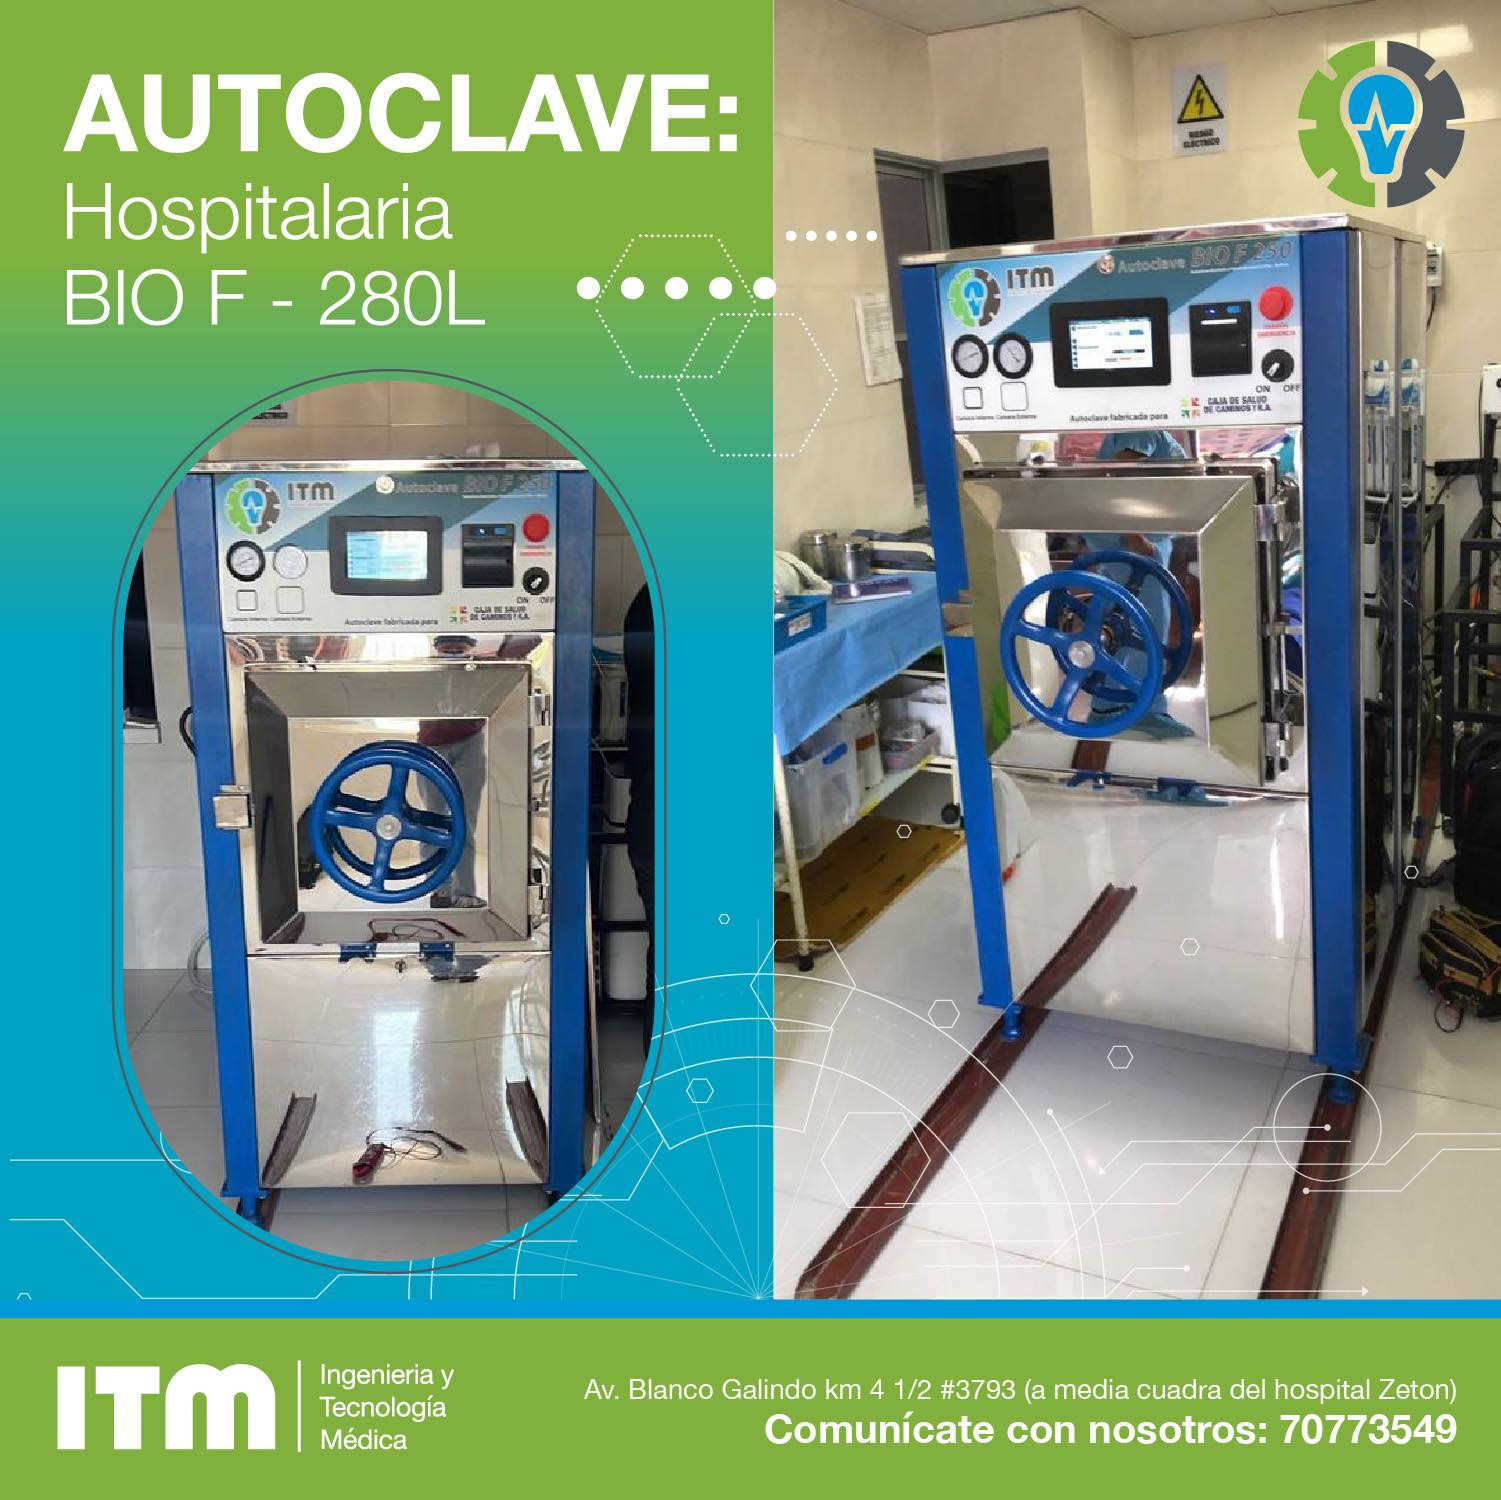
\includegraphics[width=0.4\columnwidth]{Figuras/autoclave-itm.jpg}}
        % separaciones | agregar una de las opciones entre cada par de imágenes
            \qquad      % figuras en la misma linea
            %\par        % siguiente línea
        % imagen 2
        \subfloat[Autoclave de sobremesa ITM]{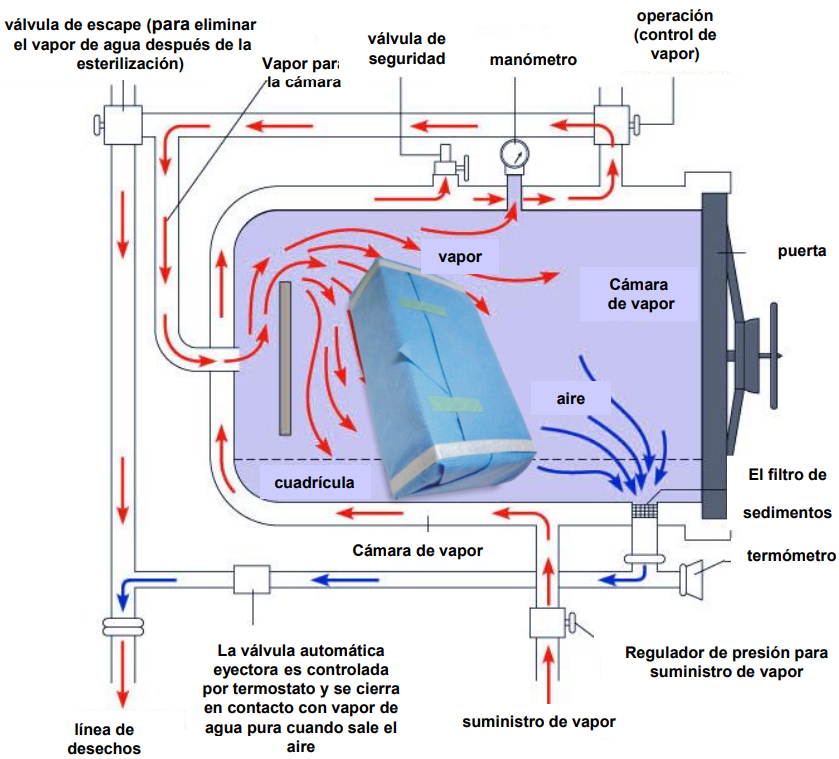
\includegraphics[width=0.4\columnwidth]{Figuras/autoclave.png}}\\
    \centering{\textbf{Fuente:} Pagina de facebook \acrshort{itm} (2024)}
    \label{fig:autoclaves}
\end{figure}

\newpage